\documentclass[twoside]{article}
\setlength{\oddsidemargin}{-0.5 in}
\setlength{\evensidemargin}{1.5 in}
\setlength{\topmargin}{-0.6 in}
\setlength{\textwidth}{5.5 in}
\setlength{\textheight}{8.5 in}
\setlength{\headsep}{0.5 in}
\setlength{\parindent}{0 in}
\setlength{\parskip}{0.07 in}
\setlength{\marginparwidth}{145pt}

%
% ADD PACKAGES here:
% 12

\usepackage{amsmath,
            amsfonts,
            amssymb,
            graphicx,
            mathtools,
            flexisym,
            marginnote,
            hyperref,
            titlesec}

\usepackage[english]{babel}
\usepackage[utf8]{inputenc}
\usepackage[shortlabels]{enumitem}

\graphicspath{ {images/} }

\hypersetup{
    colorlinks=true,
    linkcolor=blue,
    filecolor=magenta,      
    urlcolor=blue,
}

\titlespacing\section{0pt}{12pt plus 4pt minus 2pt}{0pt plus 2pt minus 2pt}
\titlespacing\subsection{0pt}{12pt plus 4pt minus 2pt}{0pt plus 2pt minus 2pt}

%
% The following commands set up the lecnum (lecture number)
% counter and make various numbering schemes work relative
% to the lecture number.
%
\newcounter{lecnum}
\renewcommand{\thepage}{\thelecnum-\arabic{page}}
\renewcommand{\thesection}{\thelecnum.\arabic{section}}
\renewcommand{\theequation}{\thelecnum.\arabic{equation}}
\renewcommand{\thefigure}{\thelecnum.\arabic{figure}}
\renewcommand{\thetable}{\thelecnum.\arabic{table}}

\newcommand{\aosv}{1044414: Advanced Operating Systems and Virtualization}
\newcommand{\wir}{1038137: Web Information Retrieval}
\newcommand{\va}{1052057: Visual Analytics}
\newcommand{\advprog}{1044416: Advanced Programming}
\newcommand{\dchpc}{1044399: Data Centers and High Perf. Computing}

\newcommand{\qu}[1]{\marginnote{\textcolor{cyan}{#1}}}


%
% The following macro is used to generate the header.
%
\newcommand{\lecture}[4]{
   \pagestyle{myheadings}
   \thispagestyle{plain}
   \newpage
   \setcounter{lecnum}{#4}
   \setcounter{page}{1}
   \noindent
   \begin{center}
   \framebox{
      \vbox{\vspace{2mm}
    \hbox to 7.4in { {\bf #1
    \hfill Spring 2018} }
       \vspace{4mm}
       \hbox to 7.4in { {\Large \hfill Lecture #4: #2  \hfill} }
       \vspace{2mm}
       \hbox to 7.4in { {\it Lecturer: #3 \hfill Scribe: Anxhelo Xhebraj} }
      \vspace{2mm}}
   }
   \end{center}
   \markboth{Lecture #4: #2}{Lecture #4: #2}

   \iffalse
   {\bf Note}: {\it LaTeX template courtesy of UC Berkeley EECS dept.}

   {\bf Disclaimer}: {\it These notes have not been subjected to the
   usual scrutiny reserved for formal publications.  They may be distributed
   outside this class only with the permission of the Instructor.}
   \vspace*{4mm}
   \fi
}
%
% Convention for citations is authors' initials followed by the year.
% For example, to cite a paper by Leighton and Maggs you would type
% \cite{LM89}, and to cite a paper by Strassen you would type \cite{S69}.
% (To avoid bibliography problems, for now we redefine the \cite command.)
% Also commands that create a suitable format for the reference list.
\iffalse
\renewcommand{\cite}[1]{[#1]}
\def\beginrefs{\begin{list}%
        {[\arabic{equation}]}{\usecounter{equation}
         \setlength{\leftmargin}{2.0truecm}\setlength{\labelsep}{0.4truecm}%
         \setlength{\labelwidth}{1.6truecm}}}
\def\endrefs{\end{list}}
\def\bibentry#1{\item[\hbox{[#1]}]}
\fi

%Use this command for a figure; it puts a figure in wherever you want it.
%usage: \fig{NUMBER}{SPACE-IN-INCHES}{CAPTION}
\newcommand{\fig}[3]{
            \vspace{#2}
            \begin{center}
            Figure \thelecnum.#1:~#3
            \end{center}
    }
% Use these for theorems, lemmas, proofs, etc.
\newtheorem{theorem}{Theorem}[lecnum]
\newtheorem{lemma}[theorem]{Lemma}
\newtheorem{proposition}[theorem]{Proposition}
\newtheorem{claim}[theorem]{Claim}
\newtheorem{corollary}[theorem]{Corollary}
\newtheorem{definition}[theorem]{Definition}
\newenvironment{proof}{{\bf Proof:}}{\hfill\rule{2mm}{2mm}}

% **** IF YOU WANT TO DEFINE ADDITIONAL MACROS FOR YOURSELF, PUT THEM HERE:

\newcommand\E{\mathbb{E}}

\begin{document}

\nocite{*}

%FILL IN THE RIGHT INFO.
%\lecture{**LECTURE-NUMBER**}{**DATE**}{**LECTURER**}{**SCRIBE**}

\lecture{\aosv}{March 23}{Alessandro Pellegrini}{7}

%\footnotetext{These notes are partially based on those of Nigel Mansell.}

% **** YOUR NOTES GO HERE:


As described, even though the Buddy Allocator is a fast algorithm to manage
memory for the kernel it still has some problems that aren't really addressed:

\begin{itemize}
    \item \textbf{Internal Fragmentation:} produced by the granularity at which
        the Buddy System works (page size). If the kernel needs just a buffer
        of size less than that of a page, it still has to allocate the page
        fully, meaning that the remaining space cannot be used by other
        allocations.

    \item \textbf{External Fragmentation:} after many allocations of small size
        it might happen that the Buddy System is not able to coalesce some
        buddies into bigger blocks of contiguous memory meaning that if at some
        time the kernel needs a large block of contiguous memory, such request
        cannot be fulfilled even if there are a set of \textit{not contiguous}
        pages that together make the size of the request.

    \item \textbf{Spinlock Contention:} the allocation in the same memory zone
        within a node is serialized since each allocation needs to acquire
        \texttt{zone_t->lock}. This can become a bottleneck if multiple kernel
        threads are trying to allocate memory.
\end{itemize}

\section{Quicklists}
\label{sec:Quicklists}

Quicklists consist in pre-allocating pages for each CPU. The list of free pages
is kept in a \textit{per-cpu variable} meaning that each CPU will have its own
variable with its own list of pages. This new technique of allocating pages
increases the parallelism of the allocation with respect to the Buddy System
since threads running on different CPUs do not have to dispute on the zone lock
but can take pages from their own free list. It was mainly used for page table
pages allocations such as \texttt{pgd_alloc} etc.

The allocation of a page through quicklists is done through the
\texttt{quicklist_alloc} function.

\begin{verbatim}
    > include/linux/quicklist.h
    static inline void *quicklist_alloc(int nr, gfp_t flags, ...) {
        struct quicklist *q;
        void **p = NULL;

        q = &get_cpu_var(quicklist)[nr];
        p = q->page;

        if (likely(p)) {
            q->page = p[0];
            p[0] = NULL;
            q->nr_pages--;
        }
        put_cpu_var(quicklist);

        if(likely(p))
            return p;

        p = (void *) __get_free_page(flags | __GFP_ZERO);
        return p;
    }
\end{verbatim}

In the allocation \texttt{get_cpu_var} is called to get the reference to the
free list assigned to the CPU the thread is currently running on. In doing
so preemption is disabled in \texttt{get_cpu_var} in order to not allow the
thread to be moved on another CPU with a reference to a variable which is
specific to the CPU it is currently running on, otherwise concurrency problem
might arise.

\texttt{q->page} is the first page of the free list. It is checked whether the
free list is empty (\texttt{NULL}) through \texttt{if(likely(p))}. The
\texttt{likely} macro informs the compiler that the flow of execution will take
the branch path meaning that \textit{likely} the code block inside the
\texttt{if} will be executed therefore the compiler should take care to optimize
the branch prediction. Inside the \texttt{if} code block the \textit{head}
(first element) of the list is taken and the pointer of the list is set to the
pointer to the next page held inside \texttt{p[0]} and the number of free pages
is decremented (\texttt{q->nr_pages--}).

Finally \texttt{put_cpu_var} will re-enable preemption. If there was indeed a
page available in the free list then it is returned, otherwise the allocation
falls back to the Buddy System through \texttt{__get__free_page()}.

Quicklists were used in the i386 architecture from kernel v. 2.6.22 up to
2.6.24.7 and have then been replaced by per-cpu pages/hot-n-cold pages.


\section{SLAB Allocator}

To make more efficient the allocation of small frequently allocated/deallocated data
structures in the kernel such as \texttt{pid, mm_struct} the
\textit{slab} allocator (and in later versions also the \textit{slob} and
\textit{slub}) was introduced.

The main goals of this new allocator are:

\begin{itemize}
    \item Amortize the internal fragmentation produced by the Buddy System
        allocator for small allocations.
    \item Improve access performance to kernel object by aligning them to L1/L2
        caches.
    \item Cache commonly used objects to alleviate the system from allocating,
        initializing and destroying objects.
\end{itemize}

\begin{center}
  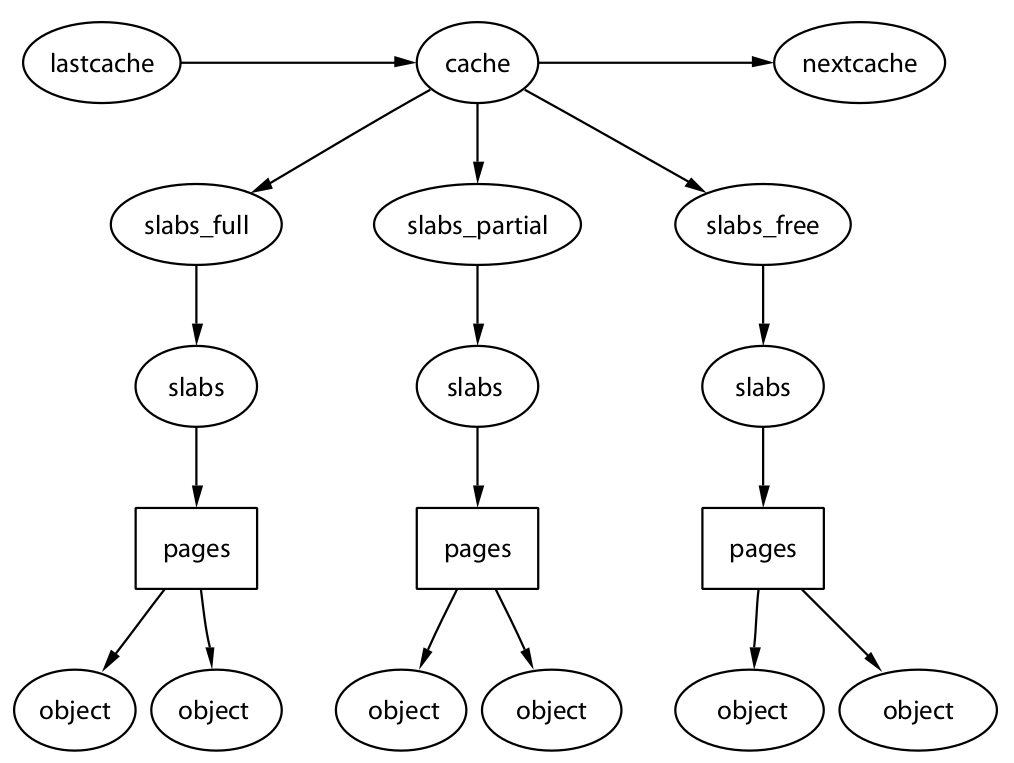
\includegraphics[width=0.8\textwidth]{slabrel.png}
  \marginnote{\fig{1}{0 pt}{Slab structs relationships. (\cite{gorman_2004} pp. 16)}}[-6cm]
\end{center}



There is a list of caches where each cache keeps a slab of a specific size. A cache is organised in three types of slabs: full (Don't have buffers to be given), partial (some used and some free), free (deallocated or never allocated). Objects are abstractions over pages.

\subsection{SLAB Interfaces}

Found in linux / malloc h. kmalloc asks for a given size and returns the virtual address of a buffer of that size. kfree frees memory allocated via kmalloc. k malloc node is an api to the slab allocator that in the end will ask to the buddy system of a specific numa node for allocating some page.  

kmalloc should be used for frequent allocations and deallocations of the same size. 

up to kernel v 3.9.11 there was the struct cache size. cs\_cachep is a pointer to the memory. There is a table of multiple size fixed-size caches. 

In kernel 3.10 we move from fixed size to list with spinlock again. You can either have a shared across cores allocator or one allocator for each core. Having one allocator for each core requires space. What's the difference btw using the buddy system and slab? buddy has one spinlock for each numa node while slab has one spinlock for each size of cache. \marginnote{SLAB and Buddy both are for the kernel}[-36 pt]

Per node cache coloring: size of object then padding and so on. Why is coloring used? to align objects to L1 Cache Bytes. Two objects of the same size will not fall in the same cache line. An object of size greater than one line is padded to the size of multiple cache lines.

This ensures that two slabs objects allocated will not fall in the same cache line to not fall into cache contention.

Members that are accessed together and used frequently together (Common Members) are placed close together to optimise cache hits for example the spinlock and slab partial in kmem cache node struct. 

(Loosely related fields): due to the false cache sharing problem we have that cache controllers in order to be coherent tell the others cache controllers that they are going to write that line wanting "mutual exclusion". With coloring we ensure that different buffers will not fall in the same cache line. 

\subsection{Cache flush operations}

Similarily to the TLB relies on the hardware specific operations for granularity and coherency of the flushing. There are also problems because the hardware cache uses virtual addresses, therefore two processes addressing the same virtual address might have a cache hit to a region of memory that is not the physical one they wanted to access. After flushing the page cache we must also flush the TLB.

\begin{description}
    \item \texttt{flush_cache_all:} Flushes the entire CPU cache system. It is used for when global data structures, for example kernel page tables, are changed to ensure cache coherency.
    \item others...
\end{description}

What is the best way to devise a cache? physical or virtual? Intel architectures use Virtual addresses to tag L1 cache. If there is a miss in L1 the TLB is consulted to get the physical and check the L2 which is addressed through the physical address. There is a protocol btw L1 and TLB to know whether a virtual address is consistent with the current paging scheme. Therefore in intel we do not care about cache consistency.

Virtual aliasing is the problem described above where we tag the L1 cache through virtual addresses but if the cache is not coherent ...

The other apis are a low level api that are used by the description above.

copy from and to user ensures that the copy of memory is done correctly since there might be a process switch and the write might be writing memory of another process.

Access ok checks whether the memory area passed is correctly mapped to that process. 

\texttt{vmalloc} used to map some memory in the kernel in a stable way, that will be used for a long time. No idea about the memory contiguousness. No info about the organisation of physical frames. Used for usually loading some kernel module for code, data etc of the module. It doesn't rely in either the Buddy system or slab. 

\texttt{virt_to_phys} and viceversa used in kmalloc or get free page to compute the mapping btw physical and virtual addresses. This is done to be hardware independent when developing a kernel module to not rely on offsets etc. 

For allocation size in kmalloc is limited to 8KB in Linux. vmalloc btw 64/128MB. Kmalloc is physical contiguous while vmalloc no. Vmalloc invalidates transparently the TLB etc while kmalloc no. This is done because for example in loading kernel modules you want that all threads have visibility of the change. 

After setting up all the memory \texttt{trap\_init()} initialises the IDT and GDT.
The only entry point to kernel land from user space is through the interrupt \texttt{0x80}. The same is done in Windows.

That interrupt executes the system call dispatcher which finds out what the user code wants to do. Every system call has a code assigned to it.

Interrupts automatically reset the Flags while Traps do not. The dispatcher explicitly clears interrupts through \texttt{cli} instruction. In multi-core systems this is not enough, we must ensure correctness of all the data structures of the kernel. Spinlocks (implemented through the \texttt{cmpxchg} instruction) are used to access data structures.

Since syscalls have preassigned numbers if we change only one of them we break backward compatibility.

Macros are used for generating asm volatile blocks defining a syscall. Multiple macros depending by the number of the parameters of the syscall (usually at most 6 parameters).

\newpage
\bibliography{Lec6}
\bibliographystyle{plainnat}
\end{document}
